\documentclass[chinese]{article}
% \usepackage{babel}
% \usepackage[hyperref=true,style=ieee]{biblatex}  % biblatex参考文献宏包
% \addbibresource{ref.bib}  % 添加引用文献bib源
\usepackage{lipsum}  % 导入生成段落的宏包
\usepackage{ctex} % 加入ctex宏包以支持中文
\usepackage{graphicx} % 加载图形处理宏包
\usepackage{booktabs} % 用于美化表格线条
\usepackage{caption} % 用于添加表格标题
\usepackage{float}
\usepackage{tabularx}
\usepackage{tcolorbox}
\tcbuselibrary{listings}
\usepackage{array}
\usepackage[dvipsnames]{xcolor}
\usepackage{tikz}
\usepackage{hyperref} 
\usetikzlibrary{positioning} % 加载positioning库
\renewcommand{\refname}{Reference}

\hypersetup{
    colorlinks=true, % 使用颜色而不是边框
    linkcolor=black, % 链接颜色为黑色
    citecolor=black, % 引用颜色为黑色
    urlcolor=blue    % URL颜色为蓝色(可以根据需要修改)
}
\lstset{
 basicstyle=\ttfamily, % 设置字体族
 breaklines=true, % 自动换行
 keywordstyle=\bfseries\color{NavyBlue}, % 设置关键字为粗体,颜色为 NavyBlue
 morekeywords={}, % 设置更多的关键字,用逗号分隔
 emph={self}, % 指定强调词,如果有多个,用逗号隔开
    emphstyle=\bfseries\color{Rhodamine}, % 强调词样式设置
    commentstyle=\itshape\color{black!50!white}, % 设置注释样式,斜体,浅灰色
    stringstyle=\bfseries\color{PineGreen!90!black}, % 设置字符串样式
    columns=flexible,
    % numbers=left, % 显示行号在左边
    % numbersep=2em, % 设置行号的具体位置
    % numberstyle=\footnotesize, % 缩小行号
    frame=single, % 边框
    framesep=1em, % 设置代码与边框的距离
	tabsize=2, % 设置tab键的宽度为2个空格
    showstringspaces=false, % 不显示字符串中的空格
}

\usepackage[margin=1in]{geometry}
\title{\textbf{ztest}: 一个快捷,易用,轻量化的C++单元测试框架}
\begin{document}
\maketitle
\tableofcontents  % 生成目录表
\newpage
\section{需求分析}%需求分析	
% As our coding abilities progress, it becomes increasingly essential to practice the skills required for constructing C++ programs. Consequently, our team has devised a plan to develop a highly user-friendly note-taking system. This system is envisioned to support a wide array of note styles, with Markdown being one of the prominent ones. It will offer users the flexibility to express their thoughts and record information in the format that suits them best. Additionally, a built-in calendar function will be incorporated to present the daily schedule. Moreover, a comprehensive file management system is also on the cards. The combination of these features is set to make our note-taking system a go-to tool for individuals seeking an efficient and versatile digital workspace.
随着复杂系统架构设计能力的培养需求日益凸显,掌握面向对象设计原则与模式化工程实践已成为高级软件工程教育的核心目标。这不仅需要理解类与对象间的动态协作关系,更要具备通过设计模式解决架构难题的抽象思维能力。
现有的单元测试框架(如Google Test)具有上手难度较高,并发支持有限,报告系统过于简洁,可拓展性一般等缺点,我们团队计划开发一个提供一个灵活、高效且易于使用(带图形用户界面GUI)的测试工具,旨在提供一个直观、易用的环境,方便开发人员和测试人员编写、运行和管理测试用例。该工具将支持多种测试类型(如单元测试、集成测试等),并提供详细的测试结果报告。
\begin{table}[h]
    \centering
    \caption{主流测试框架对比}
    \label{tab:compare}
    \begin{tabularx}{\textwidth}{lXXXX}
        \toprule
        \textbf{框架}            & \textbf{GUI支持} & \textbf{并发测试} & \textbf{报告系统} & \textbf{扩展性} \\
        \midrule
        Google Test(C++)       & 无              & 有限            & 基础            & 中等           \\
        JUnit    (Java)        & Eclipse插件      & 支持            & HTML/XML      & 高            \\
        PyTest (Python)        & 第三方工具          & 优秀            & 丰富            & 优秀           \\
        Catch2   (C++)         & 无              & 一般            & 简洁            & 中等           \\
        \textbf{Ours}    (C++) & 有              & 优秀            & 丰富            & 高            \\
        \bottomrule
    \end{tabularx}
\end{table}
% \subsection{System Objectives}%系统目标
% A note-taking system with user-friendly UI supporting markdown format. We use xmake for the management of the whole project and imgui for UI design, introducing glew, cmark dynamic link libraries and OpenGL library. And we use xmake b for compiling and xmake r for running.
%这是一个拥有用户友好型用户界面且支持 Markdown 格式的笔记记录系统。我们使用 xmake 来管理整个项目,使用 ImGui 进行用户界面设计,同时引入了 GLEW、cmark 动态链接库以及 OpenGL 库。此外,我们使用 “xmake b” 命令进行编译,使用 “xmake r” 命令来运行程序。
\section{系统功能}
本测试框架的设计目标是提供一个灵活、高效且易于使用(带图形用户界面GUI)的测试工具,支持测试用例的管理、断言验证、测试执行以及结果报告。以下将从测试用例管理、断言机制、测试执行器和结果报告四个方面详细介绍其功能。

\subsection{测试用例管理}
测试用例管理是测试框架的核心功能之一,支持测试用例的定义、注册和组织。测试用例可以通过继承基类或使用工厂模式创建,并支持设置前置和后置钩子函数。

\subsubsection{单个测试用例的创建}

实现了三种方式创建测试用例,分别为链式创建,宏定义,继承定义:

\begin{enumerate}
    \item \textbf{链式创建}: 通过链式创建,实现测试用例的自定义,在网络编程的测试中,使用链式创建的方式创建测试用例会更加符合逻辑。例子如下
          \begin{lstlisting}[language=C++]
auto test_case = TestFactory::createTest("Add", ZType::Z_SAFE, "", add, 2, 3)
                 .setExpectedOutput(5)
                 .beforeAll([]() { logger.info("Init\n"); })          
                 .afterEach([]() { logger.info("Clean\n"); }).build();
                \end{lstlisting}
    \item \textbf{宏定义}:通过宏定义,实现测试用例的自定义。宏定义极大地简化了语法,使得测试用例的定义更加清晰和结构化。展开之后实际上是继承定义+自动注册。
          \begin{lstlisting}[language=C++]
ZTEST_F(BasicMath, FailedAdditionTest) {
    EXPECT_EQ(6, add(2, 3));
    ASSERT_TRUE(6==add(2, 3));
    return Zstate::Z_SUCCESS;//如果能运行要此处,说明测试成功
}
                \end{lstlisting}
    \item\textbf{继承定义}:通过继承测试基类,实现测试用例的自定义,可拓展性更高,可以定义更多自定义的测试方法。
          \begin{lstlisting}[language=C++]
class MathTests_Addition : public ZtestBase {
    public:
        MathTests_Addition() : ZtestBase("MathTests.Addition", ZType::ZSAFE, "Test addition function") {}
        Zstate run() override {
                EXPECT_EQ(5, add(2, 3)); // 预期结果为5
                EXPECT_EQ(0, add(0, 0)); // 预期结果为0
                return Zstate::Z_SUCCESS;
        }
};
\end{lstlisting}
\end{enumerate}
\subsubsection{测试用例的注册}在宏定义的情况下可以使用测试注册中心 \textbf{ZTestRegistry} 动态注册测试用例,对于继承测试基类,由于其给予用户的自由度较高,安全起见要求用户手动添加。而链式创建的测试用例可以调用在build后调用注册函数实现注册或者手动添加。
下面是测试注册中心类的使用示例:
\begin{lstlisting}[language=C++]
// 手动注册示例
ZTestRegistry::getInstance().registerTest(std::make_shared<MathTests_Addition>());

\end{lstlisting}
\newpage
\subsubsection{测试套件的构建}
通过 \textbf{ZTestSuite} 类组织多个测试用例,支持批量运行,支持多线程测试,会统计测试多个测试用例所需的时间,测试通过的结果,通过测试数量等值。

\begin{lstlisting}[language=C++]
auto mathSuite = std::make_unique<ZTestSuite>("Math", ZType::Z_SAFE,"math test");
// 添加单测用例到套件
mathSuite->addTest(TestFactory::createTest("Addition", ZType::Z_SAFE, "", add, 2, 3).setExpectedOutput(5).build());
mathSuite->addTest(TestFactory::createTest("Subtraction", ZType::Z_SAFE, "", subtract, 5, 3).setExpectedOutput(2).build());
\end{lstlisting}



\subsection{断言机制}
断言机制用于验证测试用例的预期结果是否正确。框架提供了多种断言宏,如 \textbf{EXPECT\_EQ} 和 \textbf{ASSERT\_TRUE},支持在测试中快速验证条件。
主要提供以下断言:
\begin{itemize}
    \item \textbf{EXPECT\_EQ}:验证两个值是否相等。
    \item \textbf{ASSERT\_TRUE}:验证条件是否为真。
\end{itemize}
使用样例如下,
\begin{lstlisting}[language=C++]
// 如果断言失败,抛出异常
EXPECT_EQ(5, add(2, 3));
ASSERT_TRUE(6==add(2, 3));
\end{lstlisting}

如果断言失败,抛出 \textbf{ZTestFailureException} 异常。同时可以通过继承 \textbf{ZTestFailureException} 异常处理函数,自定义异常处理逻辑。


\subsection{测试执行器}
测试执行器负责管理测试用例的运行,支持\textbf{多线程}并行执行测试用例,并收集测试结果,实现了自动调度测试和测试结果统计。

\textbf{ZTestContext}用于测试上下文管理类,负责维护测试用例队列,并通过多线程并行执行测试。
\begin{lstlisting}[language=C++]
//定义一个测试上下文对象
ZTestContext context;
// 将测试用例添加到测试队列
for (auto &&test : registeredTests) 
    context.addTest(std::move(test));
// 多线程执行测试用例
context.runAll();
\end{lstlisting}

实际上一共可以定义两种类型的测试用例,一种是\textbf{z\_safe}类型的测试用例,一种是\textbf{z\_unsafe}型,
两种类型分别对应两种测试模式,\textbf{z\_safe}类型的测试用例是线程安全的,
\textbf{z\_unsafe}类型的测试器是线程不安全的,默认为\textbf{z\_safe}类型。
如果测试时候有\textbf{z\_unsafe}类型出现,则会等待其执行完成,再执行\textbf{z\_safe}类型的测试用例。

\subsection{结果报告}
\subsubsection{报告文件保存}
测试完成后,框架会生成详细的测试结果报告,包括测试名称、运行时间、通过/失败状态以及错误信息。
我们定义评测结果状态有三种状态:
\begin{itemize}
    \item \textbf{z\_success}:测试通过。
    \item \textbf{z\_failed}:测试失败。
    \item \textbf{z\_unknown}:还没有完成测试。
\end{itemize}
\textbf{日志输出}测试结果通过 \textbf{ZLogger} 类输出到控制台或文件中。
输出规则如下,
[   info   ]表示测试信息,[   FAILED  ]表示测试失败,[   OK   ]表示测试成功。
输出示例如下:
\begin{lstlisting}[language=C++]
    [    OK    ] BasicMath.NegativeTest (0 ms)
    [   info   ]准备加法测试环境...
    [    OK    ] Advanced.Multiplication (0 ms)
    [  FAILED  ] BasicMath.FailedSubtractionTest (1 ms)
    Error: Test Failure in BasicMath.FailedSubtractionTest:
      Expected: 3
      Actual  : 2
    [  FAILED  ] BasicMath (1 ms)
\end{lstlisting}
同时在\textbf{ZTestResult}类中,保存了测试的运行时间,测试通过/失败状态,错误信息等信息,用来保存测试结果。
\newpage
\subsubsection{GUI展示}
可以通过GUI展示测试结果,同时未来考虑在GUI界面加入添加测试用例,删除测试用例,修改测试用例,导出测试报告等功能,界面设计大体如下图所示。
\begin{figure}[H]
    \centering
    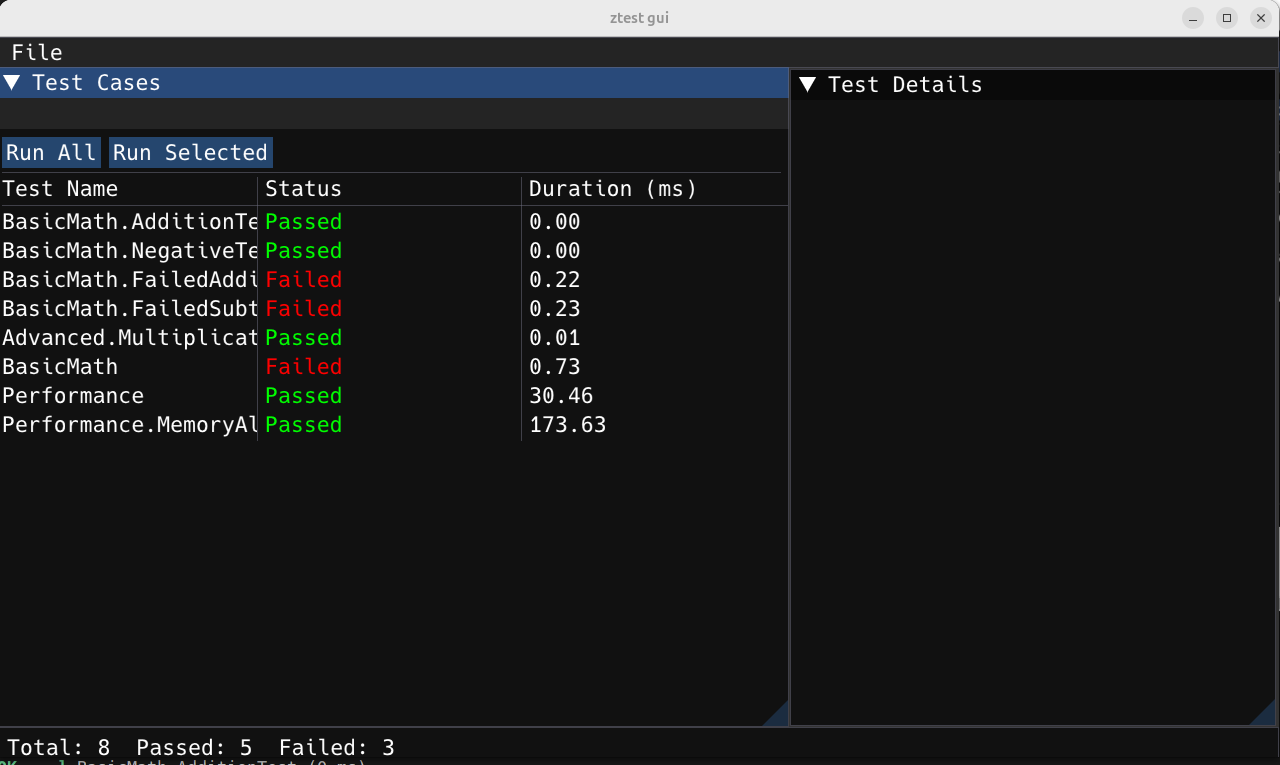
\includegraphics[width=\textwidth]{img/gui.png}
    \caption{测试管理界面布局示意图}
    \label{fig:gui}
    \small
\end{figure}

% \section{技术选型}
% \begin{table}[H]
%     \centering
%     \caption{Development Environment Configuration}
%     \begin{tabular}{@{}lc@{}} % 去掉表格左右的多余间距
%         \toprule
%         \textbf{Component} & \textbf{Tool Used for Development} \\
%         \midrule
%         Compiler           & Clang                              \\
%         Graphics API       & OpenGL                             \\
%         GUI Framework      & Dear ImGui                         \\
%         Markdown Parser    & cmark                              \\
%         Server             & Python, Flask                      \\
%         Upload Tool        & libcurl                            \\
%         Plugin System      & Lua/Python                         \\
%         PDF Generation     & Pandoc                             \\
%         Build System       & XMake                              \\
%         \bottomrule
%     \end{tabular}
% \end{table}
% \subsection{GUI框架}
% 市面上存在的C++实现markdown笔记软件使用的GUI框架多为QT,例如vnotex/vnote,nuttyartist/notes等。选取这个框架的原因是QT库中qt webengine可以很方便地使用封装的Chromium实现markdown的渲染。
% 但是这个方案存在编译后文件大,框架本身过于臃肿等问题。作为高级程序设计的课设,使用这一高度封装的技术显然过于简单,对于如何在程序中使用高级程序设计并没有帮助。

% 所以我们决定使用imgui框架。相较于QT,该框架具有轻量级,高效,可定制性强等优点。同时该框架虽然在开源社区有较高热度,但是还没有现成的markdown笔记软件被开发出来,所以其意义比重新开发一个已经较为成熟的QT笔记软件要来的大的多。从学习的角度来讲,使用该框架可以让我们更加深入的了解GUI框架底层的实现方法。
% \subsection{构建系统}
% 考虑到cmake极高的学习成本和冗余且笨重的语法,我们决定使用xmake来实现作为构建系统。
% xmake 是一个基于 Lua 的轻量级跨平台构建工具,使用 xmake.lua 维护项目构建,相比 makefile/CMakeLists.txt,配置语法更加简洁直观,对新手非常友好,短时间内就能快速入门,能够让我们把更多的精力集中在实际的项目开发上。
% \subsection{markdown解析}
% 由于markdown解析属于是编译原理课程的内容,我们认为自己在本门课重新实现意义不大,所以选取了cmark工具将markdown源码解析到AST(抽象语法树)。
% \subsection{服务端}
% 在云端服务器的实现并不是本工具的核心,所以使用python和flask库作简单实现。实际上可以替换成自己写的用C++编写服务器。(如果有实现服务器端代码的小组,可以合作的)

% 但是本地和服务器的通信使用的是libcurl(C++库)。libcurl 是一个广泛使用的、支持多种协议的、开源的客户端URL传输库,提供了许多用于数据传输的API,例如文件传输、FTP、HTTP、HTTPS、SMTP等。

% \subsection{插件系统}
% 使用C++链接动态库的实现,在linux使用dlfcn.h实现。后续考虑使用lua或者python语言实现插件。
\newpage
\section{整体架构}
核心模块上我们通过插件模式加载测试用例和待测函数。核心模块分为四个部分。
\begin{figure}[H]
    \centering
    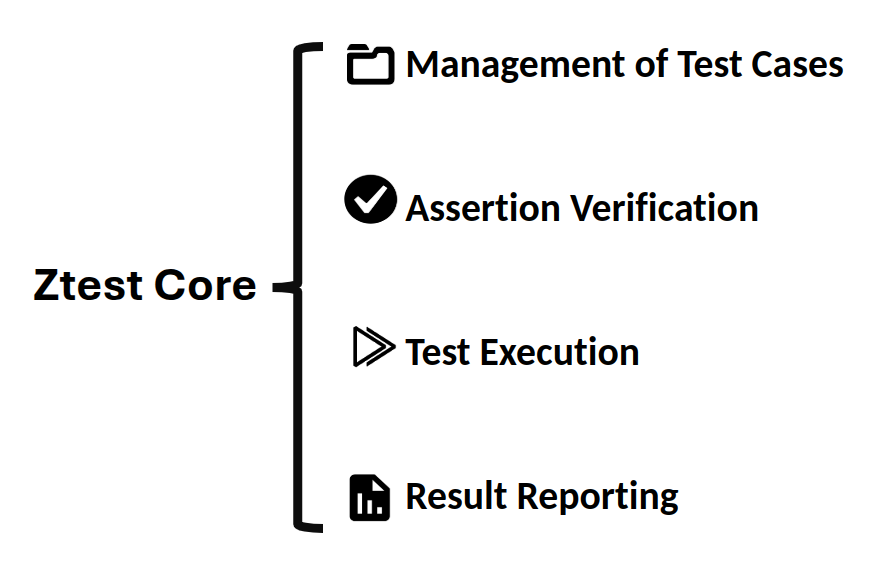
\includegraphics[width=0.6\textwidth]{img/ztest.png} % 插入图片
    \caption{ ztest core architecture}
    \label{fig:ztest core architecture}
\end{figure}

GUI整体架构上使用的是MVC(Model-View-Controller)模式架构。View关注用户所看见的UI并且提供交互,Controller负责控制器作用于模型和视图上。它控制数据流向模型对象,并在数据变化时更新视图。它使视图与模型分离开。Model主要实现对于底层文件的建模。
\begin{figure}[H]
    \centering
    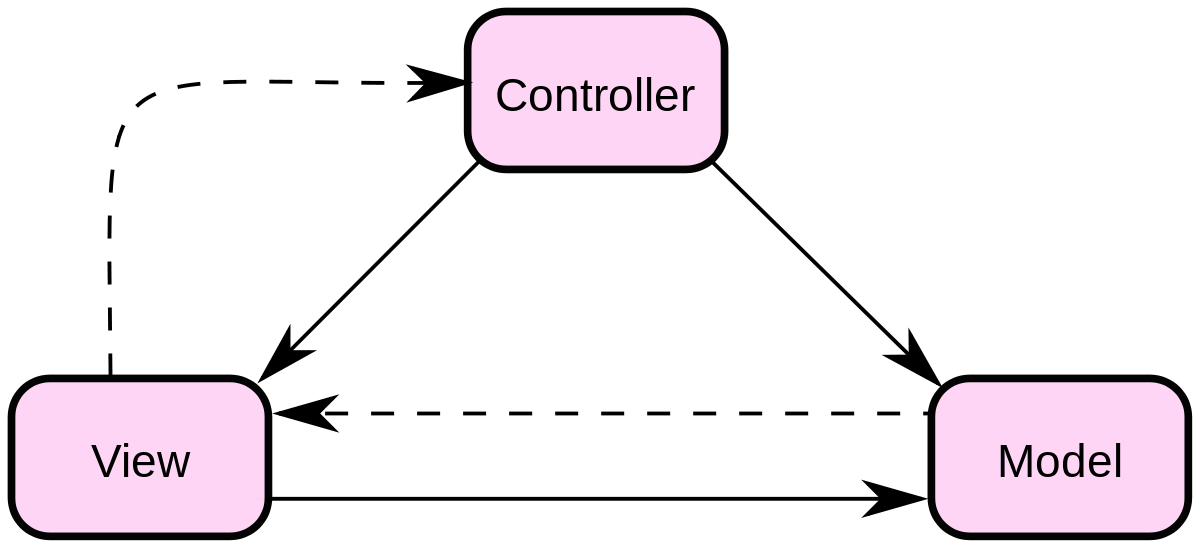
\includegraphics[width=0.8\textwidth]{img/mvc.png} % 插入图片
    \caption{ ztest gui architecture}
    \label{fig:mvc}
\end{figure}
\section{技术细节}
\subsection{测试框架设计}

\begin{itemize}
    \item \textbf{ZtestInterface}:定义了测试用例的基本接口,包括获取测试名称、运行测试以及获取测试类型等方法。
    \item \textbf{ZtestBase}:作为测试用例的基类,实现了测试的基本属性和方法,如测试名称、测试类型、描述信息、前置钩子函数(beforeAll)和后置钩子函数(afterEach)等。
    \item \textbf{ZtestSingleCase}:继承自 \textbf{ZtestBase},用于定义单个测试用例。支持设置测试函数、预期结果以及描述信息,并实现了测试的执行逻辑。
    \item \textbf{ZTestSuite}:用于组织多个测试用例,支持批量运行测试,并统计测试结果(通过、失败、总耗时等)。
    \item \textbf{ZTestRegistry}:采用单例模式实现的测试注册中心,负责注册和管理测试用例,支持动态添加测试用例。
    \item \textbf{ZTestContext}:测试上下文管理类,负责维护测试用例队列,并通过多线程并行执行测试用例,同时收集和管理测试结果。
\end{itemize}

\subsection{测试用例的构建与执行}
测试用例的构建通过 \textbf{TestBuilder} 类实现,支持链式调用设置测试函数、预期结果、前置钩子和后置钩子等。测试工厂类 \textbf{TestFactory} 提供了创建测试用例的便捷方法。

测试执行时,\textbf{ZTestContext} 类会从测试队列中取出测试用例,并通过 \textbf{ZTimer} 类计时,记录测试的开始时间、结束时间和耗时。测试结果通过 \textbf{ZTestResult} 类封装,并在控制台输出测试结果的详细信息。

\subsection{测试断言与异常处理}
框架提供了断言宏 \textbf{EXPECT\_EQ} 和 \textbf{ASSERT\_TRUE},用于比较预期值和实际值,或验证条件是否为真。如果断言失败,会抛出 \textbf{ZTestFailureException} 异常,并记录错误信息。

\subsection{测试套件与多线程执行}
测试套件(\textbf{ZTestSuite})可以包含多个测试用例,并支持批量运行。测试上下文(\textbf{ZTestContext})通过多线程并行执行测试用例,充分利用多核 CPU 的计算能力,提高测试效率。

\subsection{日志管理}
框架通过 \textbf{ZLogger} 类提供日志功能,支持线程安全的日志输出。日志信息包括测试结果、错误信息以及测试用例的前置和后置操作信息。


\subsection{UI 实现}
本系统采用 MVC 架构实现图形用户界面,通过 Dear ImGui 框架构建可视化测试管理界面。UI 模块的核心组件包括模型管理、视图渲染和控制器交互三部分,具体实现如下:

\subsubsection{模型管理类 (\textbf{ZTestModel})}
\textbf{ZTestModel} 维护测试用例的状态信息(名称、状态、耗时、错误信息),提供线程安全的数据更新接口 \texttt{updateFromContext()},记录当前选中测试用例 \texttt{\_selected\_test},并跟踪测试运行状态 \texttt{\_is\_running} 和进度 \texttt{\_progress}。

\subsubsection{视图渲染类 (\textbf{ZTestView})}
\textbf{ZTestView} 负责渲染用户界面,包括主菜单、测试列表窗口和详情窗口。主菜单渲染 (renderMainMenu) 实现文件菜单退出功能。测试列表窗口 (renderTestList) 采用三栏式布局显示测试名称、状态和耗时,支持测试用例选择交互,并提供「全部运行」和「运行选中」操作按钮。详情窗口 (renderDetailsWindow) 显示选中测试的详细信息,包含错误消息的多行文本展示,并使用颜色编码(绿色表示成功,红色表示失败)标识状态。

\subsubsection{控制器类 (\textbf{ZTestController})}
\textbf{ZTestController} 实现测试执行的线程管理,提供 \texttt{runAllTests()} 和 \texttt{runSelectedTest()} 方法,处理多线程与模型状态的同步。



\begin{figure}[H]
    \centering
    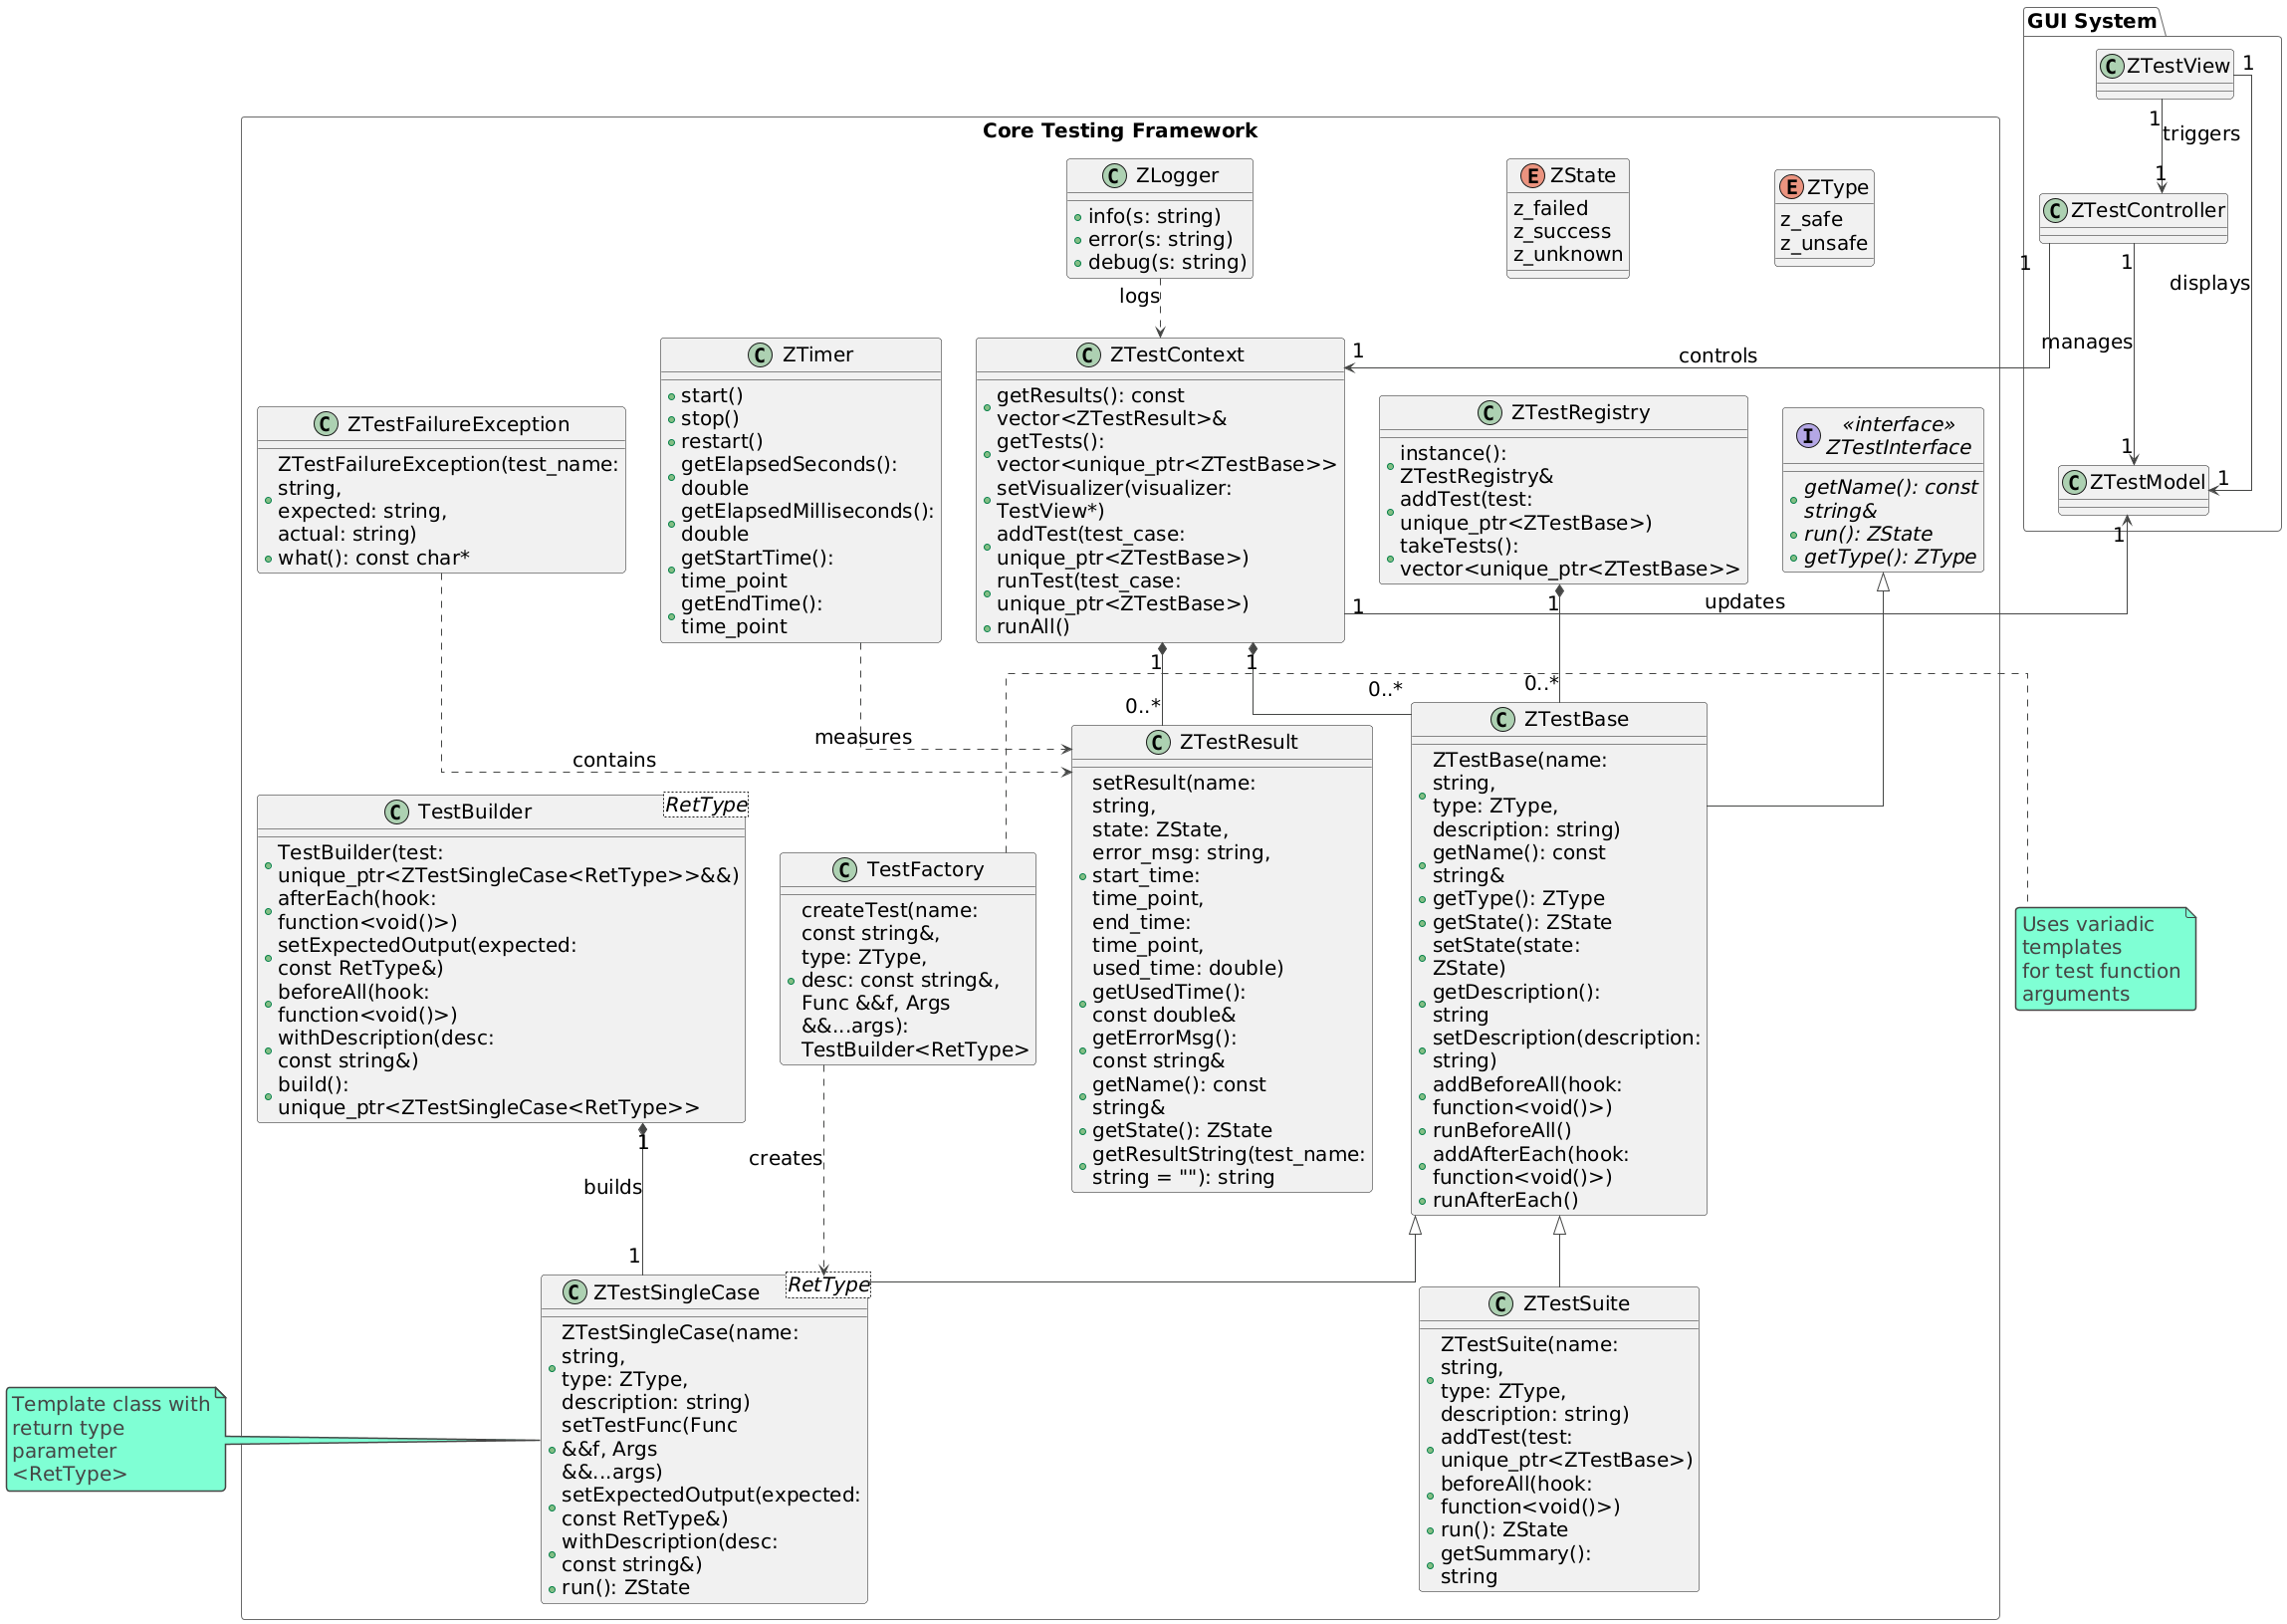
\includegraphics[angle=270,width=0.95\textwidth]{img/umlcore.png} % 插入图片
    \caption{ uml class diagram}
    \label{fig:diagram}
\end{figure}
\begin{figure}[H]
    \centering
    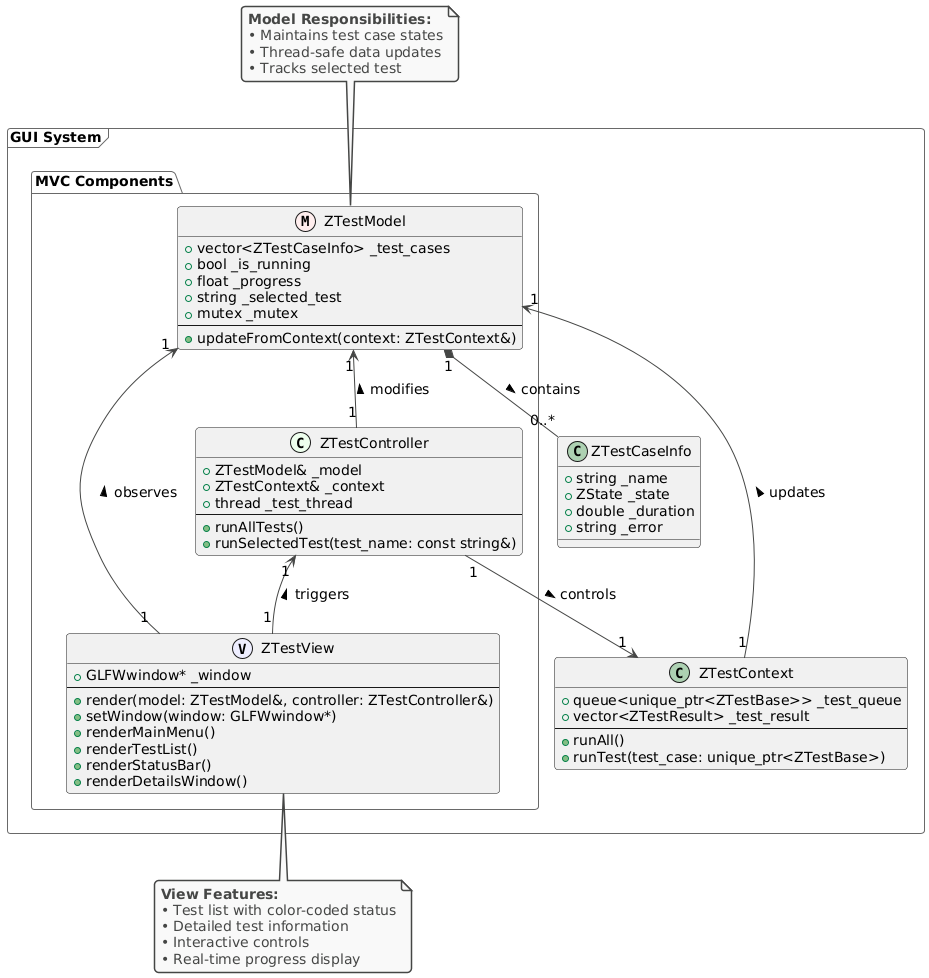
\includegraphics[angle=270,width=\textwidth]{img/umlgui.png} % 插入图片
    \caption{ gui类图}
    \label{fig:diagram}
\end{figure}
\newpage
% \begin{figure}[H]
%     \centering
%     \includegraphics[angle=270,width=0.88\textwidth]{img/UI.png} % 插入图片
%     \caption{UI  class diagram}
%     \label{fig:UI diagram}
% \end{figure}

\section{系统关键难点}
\subsection{待测函数的自动类型推导}
我们设计在使用\textbf{ZtestSingleCase}时候,用户只需要传入函数名、参数和期望结果,就可以由\textbf{ZtestSingleCase}接管运行的具体逻辑和测试结果的比较。
这要求我们在构建\textbf{ZtestSingleCase}的时候,实现自动推导待测函数的参数类型,返回值类型,以便调用函数用于测试和测试结果验证。主要使用泛型和闭包实现。
\subsection{待测试文件和测试文件的分离和动态加载}
在简单的测试中,似乎不分离待测文件和测试文件的问题不大。但是当待测项目的规模不断增大,项目的测试用例也变多时,如果仍然不分离,代码的维护和修改将非常麻烦。
作为测试框架,我们需要提供将待测文件和测试文件分离的能力,将测试文件放入\textbf{test}文件夹下,待测文件放入\textbf{src}文件夹下。
我们设计的是用户可以通过动态库链接的方式,实现测试执行。从更高的视角来看,此处我们的GUI测试框架相当于是主程序,而用户的待测代码和测试用例相当于插件。我们需要提供接口\textbf{ZTestAPI},使得主程序可以调用插件函数(测试文件和待测文件中的函数)。
\begin{figure}[H]
    \centering
    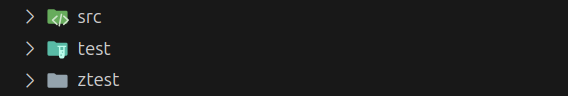
\includegraphics[width=\textwidth]{img/file.png} % 插入图片
    \caption{ 目录文件结构}
    \label{fig:diagram}
\end{figure}
\begin{lstlisting}[language=C++]
//待测试函数导出示例
ZTestAPI int subtract(int a, int b) { return a - b; }
\end{lstlisting}
\subsection{多种构建方式的实现}
实现多种测试用例构建方式,实际上是为了为用户提供更好的体验。从实现上来说,链式创建构建主要使用了builder设计模式,单个测试用例的创建主要使用了工厂模式。而宏定义实现主要使用了将宏展开到继承定义。多种语法的实现方便了用户,但是如何将这些语法构建的类统一的管理又是一个难点。
\begin{figure}[H]
    \centering
    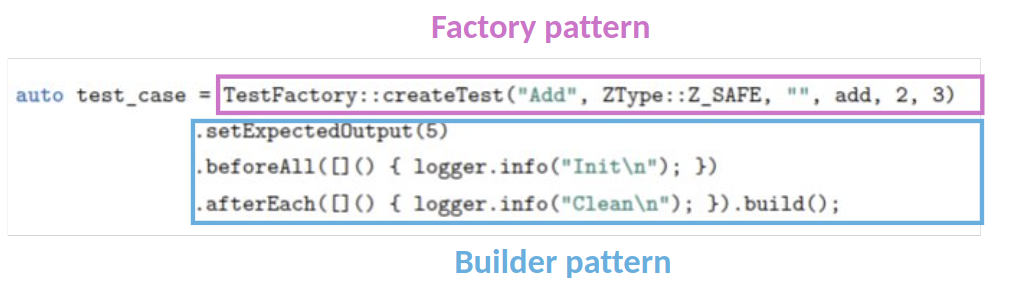
\includegraphics[width=\textwidth]{img/build.png} % 插入图片
    \caption{ 实现链式创建}
    \label{fig:diagram}
\end{figure}
\subsection{安全的多线程评测的实现}
实际上并不是所有的函数都是多线程安全的,所以我们需要对于待测函数进行分类,分别进行多线程安全的评测。实际上一共可以定义两种类型的测试用例,一种是\textbf{z\_safe}类型的测试用例,一种是\textbf{z\_unsafe}型,
两种类型分别对应两种测试模式,\textbf{z\_safe}类型的测试用例是线程安全的,
\textbf{z\_unsafe}类型的测试器是线程不安全的,默认为\textbf{z\_safe}类型。
如果测试时候有\textbf{z\_unsafe}类型出现,则会等待其执行完成,再执行\textbf{z\_safe}类型的测试用例。
\begin{figure}[H]
    \centering
    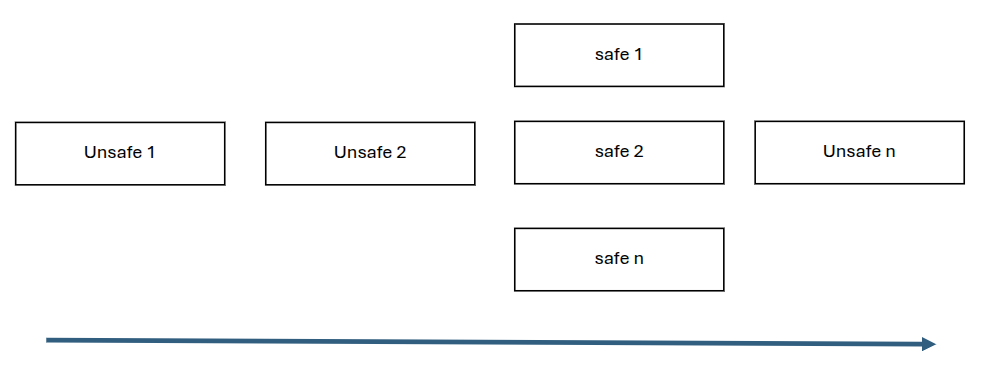
\includegraphics[width=\textwidth]{img/run.png} % 插入图片
    \caption{实现安全的多线程运行}
    \label{fig:diagram}
\end{figure}
\subsection{测试结果数据存储}
我们使用了多线程评测以后,每次评测的顺序都不一定是一样的,但是我们不希望每一次评测的结果都是不一样的顺序显示在GUI上,同时我们还希望对历史测试结果进行存储,否则会极大降低用户体验。从设计的角度来看,我们应当增加一个中间层,更加确切地说,我们可能需要在中间添加一个类似于数据库的模块,来存储测试结果,并且为\textbf{ZTestModel}使用。
\subsection{指针的管理}
考虑到本框架使用了大量的指针,很容易就会出现内存泄漏等问题,所以我们决定使用C++11中的智能指针来管理内存,来提升系统的可靠性。
\begin{table}[H]
    \centering
    \caption{详细责任分工与技术实现要点}
    \label{tab:division}
    \begin{tabularx}{\textwidth}{>{\centering\arraybackslash}m{3cm}>{\centering\arraybackslash}m{3cm}}
        \toprule
        \textbf{功能模块} & \textbf{负责人} \\
        \midrule
        GUI 实现        & 吴泓庆          \\
        断言机制          & 王瑞箐          \\
        测试用例管理        & 郑辰阳、叶穗华      \\
        测试用例执行        & 郑辰阳          \\
        报告结果生成        & 齐彦淞          \\
        \bottomrule
    \end{tabularx}
\end{table}

\centering
\textbf{职责描述与实现细节}
\begin{description}
    \item[GUI 实现]
          \begin{itemize}
              \item 基于Dear ImGUI框架构建可视化界面
              \item 实现测试列表的三栏布局(名称/状态/耗时)
              \item 开发进度条组件与状态栏实时更新
              \item 实现测试详情窗口的错误信息渲染
          \end{itemize}
    \item[断言机制]
          \begin{itemize}
              \item 设计类型安全的模板化断言宏(EXPECT\_EQ/ASSERT\_TRUE)
              \item 实现彩色错误输出
              \item 开发可扩展的异常处理框架(ZTestFailureException)
              \item 支持自定义比较算子的注册机制
          \end{itemize}
    \item[测试用例管理]
          \begin{itemize}
              \item 构建链式API(TestBuilder)实现流畅接口
              \item 开发宏展开系统(ZTEST\_F)实现自动注册
              \item 设计测试套件(ZTestSuite)的树形组织结构
              \item 实现前置/后置钩子的依赖注入机制
              \item 开发插件式测试加载系统(动态库集成)
          \end{itemize}
    \item[测试用例执行]
          \begin{itemize}
              \item 构建线程池调度器(ZTestContext)
              \item 实现安全/非安全测试的隔离执行策略
              \item 设计测试优先级队列与超时终止机制
          \end{itemize}
    \item[报告结果生成]
          \begin{itemize}
              \item 设计结构化结果存储格式(ZTestResult)
              \item 实现ANSI转义码的彩色控制台输出
              \item 构建历史测试结果的版本对比系统
              \item 集成数据可视化组件(图表生成)
          \end{itemize}
\end{description}

\newpage
\begin{thebibliography}{99}

    \bibitem{googletest}
    GoogleTest - Google Testing and Mocking Framework.
    \url{https://github.com/google/googletest}.
    Accessed: 2025-04-27.

    \bibitem{junit5}
    JUnit 5 - The 5th major version of the programmer-friendly testing framework for Java and the JVM.
    \url{https://github.com/junit-team/junit5}.
    Accessed: 2025-04-27.

    \bibitem{pytest}
    The pytest framework makes it easy to write small tests, yet scales to support complex functional testing.
    \url{https://github.com/pytest-dev/pytest}.
    Accessed: 2025-04-27.

    \bibitem{catch2}
    Catch2 - A modern, C++-native, test framework for unit-tests, TDD and BDD.
    \url{https://github.com/catchorg/Catch2}.
    Accessed: 2025-04-27.

    \bibitem{googletestuserguide}
    GoogleTest User’s Guide.
    \url{https://google.github.io/googletest/}.
    Accessed: 2025-04-27.

\end{thebibliography}

\end{document}